\section{Kubernetes}
\label{01:sec:title}

In 2014, Google came with a new concept of container management.
This concept has opened the door for many products to simplify their management of applications deployments.
This technology defined a set of primitives, which collectively provide mechanisms that deploy, maintain and scale applications based on CPU, memory, or custom metrics.
Moreover, it does not create a virtual machine but uses the kernel of the physical computer.
Also known as the lightweight approach compared to virtual machines.
Kubernetes follows leader and follow architecture.
The leader node controls Kubernetes resources and the follow node is responsible for resource creation.
The definition of these resources is given in a declarative way using YAML\footnote{YAML
\---\ human-readable serialization format (\url{https://yaml.org/})} formatted files.

\subsection{History}
\label{fig:history}

So far, we have developed four approaches to managing applications on the top of the operating system \cite{history}.
In each direction, we have eliminated certain disadvantages based on empirical knowledge.

\begin{enumerate}
    \item \textbf{Ruuning a psysical machine}\,---\,The first phase of how to deploy applications was to execute the program on the physical computer.
    This approach was not as practical as it seemed at first.
    The main issues were scalability, management of hardware, security, and price.
    Besides that, sharing memory between five running applications in an identical environment is not ideal.
    Moreover, to isolate the applications from one another, one has to buy five physical servers, significantly increasing costs.

    \item \textbf{Virtualization}\,---\,The next phase has solved problems like scalability, security, and also price.
    This allows an application to run on a single machine without sharing memory, which means it is isolated and encapsulated from other applications.
    Furthermore, you can run many of these virtual machines on a single physical server, and your only limitations are the server resources.
    These virtual machines are independent of each other, and therefore the security is much higher.
    However, resource consumption is still high since each virtual machine includes a full operating system.
    At the same time, the management of these entities is not easy if we imagine production with hundred virtual machines.
    Another limitation is, that sometimes applications need to share information with each other and the strong isolation of VMs makes this difficult.

    \item \textbf{Containerization}\,---\,In the last phase, containerization is considered as a lightweight alternative to virtualization.
    The difference between these two phases is that virtualization is using hypervisors\footnote{Hypervisor - It is a software that manages virtual machines, for instance, VMware or VirtualBox.} to manage all the virtual machines which have operating systems. The container shares the operating system with the server. Similar to virtualization, they have their filesystem, memory, and space. Containerization has become the most popular technology due to the several benefits it offers:
    \begin{itemize}[itemsep=1mm, parsep=0pt]
        \item \textbf{Isolation} \---\ predictable application performance,
        \item \textbf{Observability} \---\ gathering of information, providing metrics, logs,
        \item \textbf{Portability} of distribution in the cloud and OS \---\ runs on basically all available OS, public clouds, and so on,
        \item \textbf{Agile approach} \---\ easy to create and manage smaller container images instead of using virtual machine images, which are usually much larger.
    \end{itemize}
    Unfortunately, containerization still has several shortcomings, such as managing more running containers simultaneously, making debugging challenging, etc.

    \begin{figure}[!ht]
        \centering
        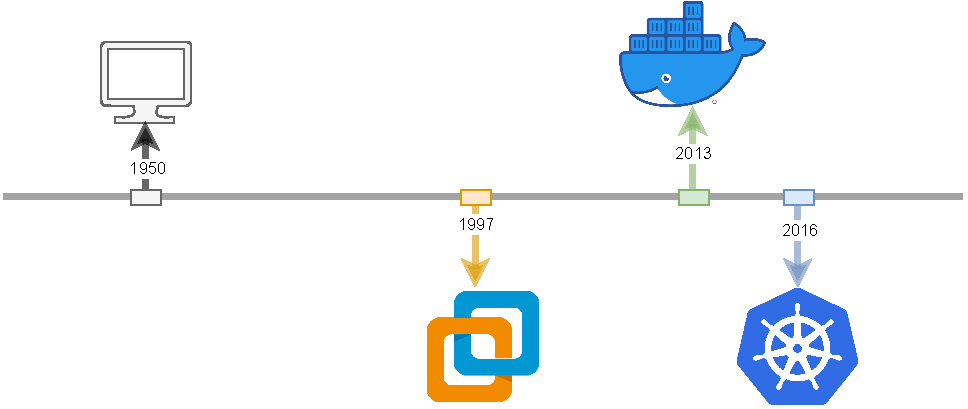
\includegraphics[scale=0.9]{obrazky-figures/02-preliminaries/01-kubernetes/01-timeline-with-picture.pdf}
        \label{01:fig:timeline}
        \caption{Evolution of virtual technologies}
    \end{figure}

    \item \textbf{Container orchestration}\,---\,The phase of the present.
    Let's imagine a situation where we run several containers and want to know the container's current state or metadata information.
    It is not straightforward to get such information because we have to look at each running container separately and analyze it.
    Kubernetes brings us a solution to this problem.
    While in containers, we have to search each one individually, so in Kubernetes, we all have it simultaneously.
    Figure \ref{01:fig:timeline} illustrates and summarises the phases of managing an application on top of the operating system, starting in 1950 when the first computer, ENIAC, was assembled—moving to the virtualization era, which started in the early 70s.
    IBM Cambridge Scientific Center began the development of CP-40, the first operating system that implemented complete virtualization.
    However, what is very important to note is that the first known virtualization software was VMware, created in 1997. Afterwards, the lightweight era comes with an idea whose functionality was based on containerization \cite{docker}.
    Finally, we have a manager who takes care of the overall management of the individual containers and guarantees their reliability, scales it effectively and more. This is what we call a container orchestration system \cite{kubernetes}.
    It has the following properties:

    \begin{enumerate}[itemsep=1mm, parsep=0pt]
        \item Deployment, StatefulSet, ReplicaSet, and Custom resource definitions (CRDs).
        \item Service and Load balancing (Service discovery).
        \item Storage (Storage orchestration).
        \item Secrets (Secret and configuration management).
    \end{enumerate}
\end{enumerate}

\subsection{Essential components of Kubernetes}
The Linux hosts can be virtual machines, bare-metal servers in the data center, or private or public cloud instances. Production environments typically have more than one master node running because of the need for High Availability\footnote{High availability (HA) \---\ is the characteristic of the system to run without failing for some period of time.}).
\begin{figure}[!h]
    \centering
    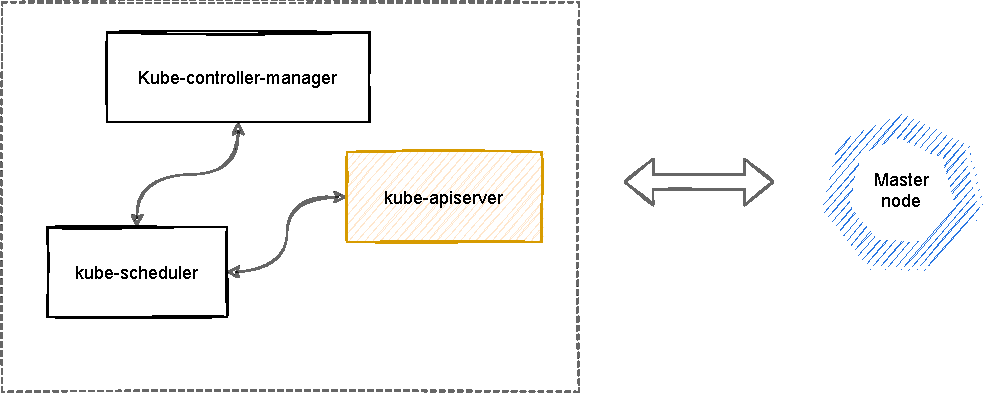
\includegraphics[scale=0.82]{obrazky-figures/02-preliminaries/01-kubernetes/02-architecture-master-sketch.pdf}
    \caption{Representation of the Master node}
    \label{02:fig:masterNode}
\end{figure}
Kubernetes services from the biggest cloud providers such as Azure Kubernetes Service (AKS), Amazon Elastic Kubernetes Service (EKS), and Google Kubernetes Service (GKS) have five master nodes, which are replicated in case of any failure.
The master node \ref{02:fig:masterNode} contains several components such as \emph{kube-controller-manager}, \emph{kube-scheduler} and \emph{kube-apiserver}.
These components are also called the "control plane".
The \emph{kube-controller-manager} takes care of all controllers where each of these controllers runs as a separate process.
The \emph{Node controller's} responsibility is to control and respond to the current status of the node.
In other words, do a health check of nodes.
There is also the \emph{Endpoint controller} for Service and Pod objects, \emph{Job controller} for Job objects, etc.
All these controllers follow algorithm \ref{01:alg:controllerAlg}.
\begin{algorithm}[H]
    \label{01:alg:controllerAlg}
    \caption{Generic algorithm for each Kubernetes controller}

    \begin{algorithmic}[1]
        \State $desired\_state \gets controller.obtain\_desired\_state()$
        \While{$True$}
            \State $desired\_state \gets controller.obtain\_desired\_state()$
            \State $current\_state\ \gets controller.observe\_current\_state()$

            \If{$current\_state \not\models desired\_state$}
                \State $controller.reconcile()$
            \EndIf

            \State $desired\_state \gets current\_state$
        \EndWhile
    \end{algorithmic}
\end{algorithm}
The \emph{kube-apiserver} works like the controller of API calls and communicates with the \emph{kube-scheduler}.
It makes sure that every created Pod is assigned to run there.
It is worthwhile to mention that we also have a component called \emph{etcd}, which works as a backup for cluster data.
Slave node components \ref{02:fig:slaveNode} suas \emph{kubelet} have taken care of containers running inside the Pod. \emph{Kube-proxy}, which reflects all the services defined in the kube-apiserver.
In the following Figure \ref{02:fig:masterAndSlaveNode}, one can see relation between master and slave nodes.

\begin{figure}[!h]
    \centering
    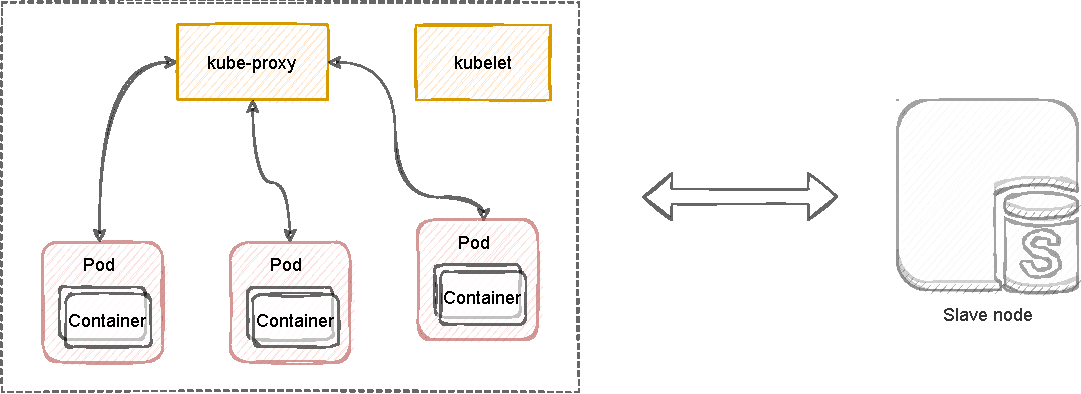
\includegraphics[scale=0.82]{obrazky-figures/02-preliminaries/01-kubernetes/02-architecture-slave-sketch.pdf}
    \caption{Representation of the Slave node}
    \label{02:fig:slaveNode}
\end{figure}


\begin{figure}[!h]
    \centering
    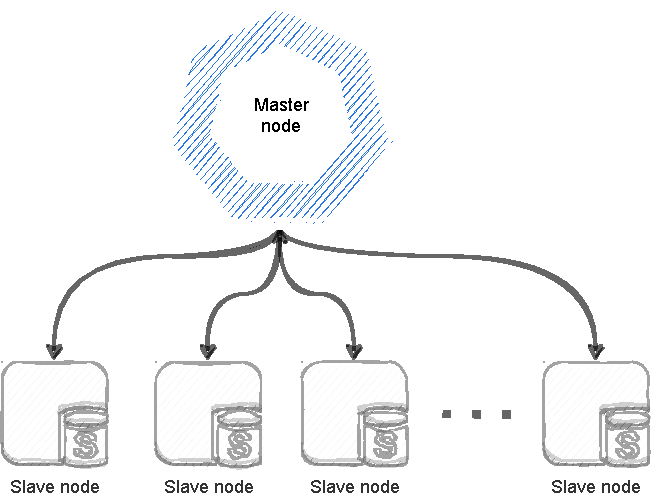
\includegraphics[scale=0.92]{obrazky-figures/02-preliminaries/01-kubernetes/02-final-architecture-master-slave.pdf}
    \caption{Relation between master and slave nodes}
    \label{02:fig:masterAndSlaveNode}
\end{figure}

\subsection{Common objects}
\label{objects}

\begin{enumerate}[itemsep=1mm, parsep=0pt]
    \item \textbf{Pod} \---\ is the atomic unit of Kubernetes.
    For instance, in the VMware environment, the atomic unit is a virtual machine, and Docker it is a container.
    The term Pod originated from the Docker logo.
    If we think about it, Docker has one whale on his logo, and we call a group of such whales Pod or, in other words, Pod of whales.
    Deductively, we can find out the property of the Pod, that is, that one or more containers can run in it.
    These containers share storage, network, and specification of how to run the container.
    If the container wants to communicate with the other container, this can be achieved using the localhost interface.
    One of the disadvantages of these resources is their lifecycle.
    If Pod crashes or is deleted, it will no longer be possible to copy this Pod.
    Instead, Kubernetes will create a new Pod with a unique ID and a new IP address assigned.

    \item \textbf{Service} \---\ represents how particular components communicate.
    Services provide reliable networking for a set of Pods.
    If Pod fails and Kubernetes creates a new Pod, its IP address is changed.
    Moreover, operations like scaling up or scaling down do the same.
    This is where Services come into play.
    They provide reliable names/alias and IP addresses.
    Furthermore, the Kubernetes service has its DNS name and port.
    It is a stable network abstraction, which provides TCP and UDP load-balancing across a dynamic set of Pods.
    By default, a service in Kubernetes has a type of \emph{ClusterIP}, which means that communication can be established only inside of the Kubernetes cluster.
    The way one can expose an application outside of the cluster is to use the following type of service which Kubernetes offers:
    \begin{itemize}[itemsep=1mm, parsep=0pt]
        \item \textbf{nodeport} \---\ exposes the service to be accessible via node IP with a specific port.
        For instance, you want to expose your HTTP server to be publicly accessible on a specific port.
        \item \textbf{load balancer} \---\  exposes the service externally using a cloud provider's load balance.
        The load balancer is shown in the definition. \emph{.status.loadBalancer} field, where you can find a real IP address.
        For example, if your demands are high and you want an application that requires more ports on specific IPs, then the usage of load balance is a wise choice.
        \item \textbf{ingress} \---\  the previously mentioned types of how to expose a service were service types, but ingress is an entry point for the cluster. \textit{It lets you consolidate your routing rules into a single resource as it can expose multiple services under the same IP address} \cite{ingress}.
    \end{itemize}

    \item \textbf{Namespace} \---\ this concept of namespaces was introduced in order to run numerous virtual clusters inside physical one. \emph{It is great for applying different quotas and access control policies. On the other hand, it is not suitable for strong workload isolation.} By default, Kubernetes starts with three initial namespaces:

    \begin{itemize}
        \item \textbf{default} \---\ the objects which do not have another namespace belongs to the default namespace,
        \item \textbf{Kube-system} \---\ namespace for objects created by the Kubernetes system, i.e. Pods, Kube-proxy, Kube-DNS. Furthermore, the service account in this namespace is used to run the Kubernetes controllers.
        \item \textbf{Kube-public} \---\ \textit{this namespace is created automatically and is recognizable by all users (including those not authenticated). In other words, there is a situation we need to have shared resources across the whole cluster; then we have to make sure that these resources are inside this namespace} \cite{namespaceTypes}
    \end{itemize}

    \item \textbf{Volume} \---\ is data storage.
    The Volume is a separated object, which binds to a Pod.
    The main ideas behind volumes are: at first, assume a scenario when your Pod crashed, and the application will lose all its data, and one would like to retrieve it secondly if one wants to share the same data between more Pods.
    The answer to these problems is the \emph{Kubernetes Volume abstraction}.
\end{enumerate}

\subsection{Controllers}

\begin{enumerate}
    \item \textbf{ReplicaSet} \---\ is the controller that is responsible for the correct number of running Pods.
    Furthermore, ReplicaSet plays a significant role in the Deployment controller, supplying a self-healing mechanism and scale operations.
    The self-healing mechanism guarantees that the Pod is running, and in the event of any error or termination of the Pod, a new one will be created immediately.
    Scale operations guarantee an easy way to increase the number of Application Pods if necessary in the event of a heavy load.
    The same applies even if the given number of Pods is already high (then we use a scale-down operation).
    ReplicaSet also has responsibility for the Rolling Update and Rollback operations available to Deployment.

    \item \textbf{Deployment} \---\ it is one of the most widely used application management controllers in the Kubernetes environment.

    \begin{figure}[!htb]
        \centering
        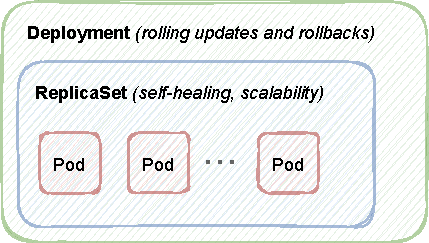
\includegraphics[scale=1.2]{obrazky-figures/02-preliminaries/01-kubernetes/03-deplyoment-archite.pdf}
        \caption{Hierarchy of Deployment, ReplicaSet and Pod inspired by The Kubernetes Book \cite{kubernetesBook}}
        \label{fig:kubernetes:deploymentReplicaSetPod}
    \end{figure}
    Based on our knowledge, the skillful reader will realize that Pod as an atomic unit will not be sufficient.
    This is mainly since Pod has no self-healing mechanism, does not support scale operations;
    Rolling Update\footnote{\textbf{Rolling Update} \---\ is the process when one updates the Deployment configuration and this update trigger replacements of the Pods with the new desired configuration} or Rollback.
    Deployment has all these features at its disposal.
    Importantly, this controller manages the ReplicaSet, which takes care of self-healing and scale operations.
    This means that the ReplicaSet checks whether the desired state is equal to the current state, such as the number of replicas are equivalent to the current state.
    Additionally, Deployment supplies the remaining properties, which are Rolling Update and Rollback.
    Since Deployment is a fully-fledged object in the Kubernetes API similar to Service, Pod, or Volume, that gives us the ability to define such an object in YAML files, such an object can then be edited and updated, which will trigger a Rolling Update.
    Figure \ref{fig:kubernetes:deploymentReplicaSetPod} shows us the hierarchy of mentioned the controllers.

    \item \textbf{StatefulSet} \---\ The last major controller is StatefulSet.
    This controller has many features in common with Deployment such as reconciliation loop described in \ref{01:alg:controllerAlg}, scaling operations, and self-healing mechanism.
    The difference between Deployment and StatefulSet are as follows:
    \begin{itemize}
        \item \textbf{storage} \---\ with the Deployment controller, it is possible to specify PersistentVolumeClaim, which is shared between all Pod replicas.
        On the other hand, in the case of StatefulSet controllers, each Pod has its own PersistentVolumeClaim.
        For clarity, one can use Deployment in the case of a stateless application, where each node does not need a unique identity, and in the case of StatefulSet, one can use it in the form of databases (i.e. Cassandra, MySQL) where each node has its own unique storage.
        \item \textbf{unique identity to Pods} \---\ in case of failure remains the same (Deployment will create a new Pod with a completely new name).
        Moreover, StatefulSet guarantees that Pods are created/deleted in order (Deployment does ensure order).
        \item \textbf{scaling operation} \---\  ensures that each new Pod is installed only after the previous one is ready and running.
        This process is repeated until we reach the number of replicas required.
        Figure \ref{02:fig:statefulsetOrderedCreation} illustrates a scaling up scenario, where firstly \emph{Pod\_1} is being deployed and after a while when \emph{Pod\_1} is running and ready, the \emph{Pod\_2} is being deployed.
    \end{itemize}

    \begin{figure}[!h]
        \centering
        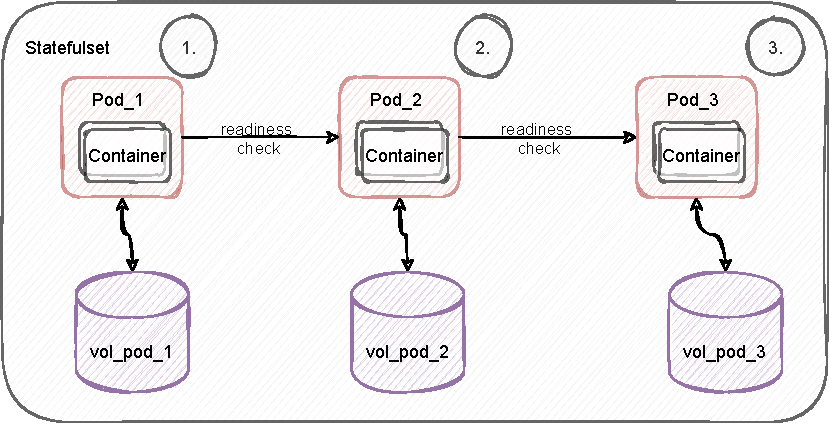
\includegraphics[scale=1]{obrazky-figures/02-preliminaries/01-kubernetes/04-statefuset_with_volume.pdf}
        \caption{StatefulSet ordered creation of Pods}
        \label{02:fig:statefulsetOrderedCreation}
    \end{figure}

    In Figure \ref{02:fig:statefulsetOrderedCreation}, we see that architecturally StatefulSets has a different self-healing and scaling operations mechanism compared to the Deployment.
    In addition, Volumes plays a significant role in the StatefulSet.
    When the Pod is created, the Statefulset immediately creates an associated volume and attaches this Volume to the Pod.
    This guarantees that the Pod can keep all its information even in the event of an unexpected failure.

\end{enumerate}